	\documentclass[12pt,twoside]{article}
%%%%%%%%%%%%%%%%%%%%%%%%%%%%%%%%%%%%%%%%%%%%%%%%%%%%%%%%%%%%%
% Meta informations:
\newcommand{\trauthor}{Miguel Angel Robles Urquiza | Rafael Ruz Gomez}
\newcommand{\trtype}{Seminar Paper} %{Seminararbeit} %{Proseminararbeit}
\newcommand{\trcourse}{Bio - Inspired Artificial Intelligence}
\newcommand{\trtitle}{Machine Learning in Chatbots}
\newcommand{\trmatrikelnummer}{7023522 | 7019703}
\newcommand{\tremail}{migueurquiza@gmail.com | rafaroco96@gmail.com}
\newcommand{\trarbeitsbereich}{Knowledge Technology, WTM}
\newcommand{\trdate}{22-12-2017}

%%%%%%%%%%%%%%%%%%%%%%%%%%%%%%%%%%%%%%%%%%%%%%%%%%%%%%%%%%%%%
% Languages:

% Falls die Ausarbeitung in Deutsch erfolgt:
% \usepackage[german]{babel}
% \usepackage[T1]{fontenc}
% \usepackage[latin1]{inputenc}
% \usepackage[latin9]{inputenc}	 				
% \selectlanguage{german}

% If the thesis is written in English:
\usepackage[english]{babel} 						
\selectlanguage{english}

%%%%%%%%%%%%%%%%%%%%%%%%%%%%%%%%%%%%%%%%%%%%%%%%%%%%%%%%%%%%%
% Bind packages:
\usepackage{acronym}                    % Acronyms
\usepackage{algorithmic}								% Algorithms and Pseudocode
\usepackage{algorithm}									% Algorithms and Pseudocode
\usepackage{amsfonts}                   % AMS Math Packet (Fonts)
\usepackage{amsmath}                    % AMS Math Packet
\usepackage{amssymb}                    % Additional mathematical symbols
\usepackage{amsthm}
\usepackage{booktabs}                   % Nicer tables
%\usepackage[font=small,labelfont=bf]{caption} % Numbered captions for figures
\usepackage{color}                      % Enables defining of colors via \definecolor
\definecolor{uhhRed}{RGB}{254,0,0}		  % Official Uni Hamburg Red
\definecolor{uhhGrey}{RGB}{122,122,120} % Official Uni Hamburg Grey
\usepackage{fancybox}                   % Gleichungen einrahmen
\usepackage{fancyhdr}										% Packet for nicer headers
%\usepackage{fancyheadings}             % Nicer numbering of headlines

%\usepackage[outer=3.35cm]{geometry} 	  % Type area (size, margins...) !!!Release version
%\usepackage[outer=2.5cm]{geometry} 		% Type area (size, margins...) !!!Print version
%\usepackage{geometry} 									% Type area (size, margins...) !!!Proofread version
\usepackage[outer=3.15cm]{geometry} 	  % Type area (size, margins...) !!!Draft version
\geometry{a4paper,body={5.8in,9in}}

\usepackage{graphicx}                   % Inclusion of graphics
%\usepackage{latexsym}                  % Special symbols
\usepackage{longtable}									% Allow tables over several parges
\usepackage{listings}                   % Nicer source code listings
\usepackage{multicol}										% Content of a table over several columns
\usepackage{multirow}										% Content of a table over several rows
\usepackage{rotating}										% Alows to rotate text and objects
\usepackage[hang]{subfigure}            % Allows to use multiple (partial) figures in a fig
%\usepackage[font=footnotesize,labelfont=rm]{subfig}	% Pictures in a floating environment
\usepackage{tabularx}										% Tables with fixed width but variable rows
\usepackage{url,xspace,boxedminipage}   % Accurate display of URLs
\usepackage{verbatim}                   % Comments

%%%%%%%%%%%%%%%%%%%%%%%%%%%%%%%%%%%%%%%%%%%%%%%%%%%%%%%%%%%%%
% Configurationen:

\hyphenation{whe-ther} 									% Manually use: "\-" in a word: Staats\-ver\-trag

%\lstloadlanguages{C}                   % Set the default language for listings
\DeclareGraphicsExtensions{.pdf,.svg,.jpg,.png,.eps} % first try pdf, then eps, png and jpg
\graphicspath{{./src/}} 								% Path to a folder where all pictures are located
\pagestyle{fancy} 											% Use nicer header and footer

% Redefine the environments for floating objects:
\setcounter{topnumber}{3}
\setcounter{bottomnumber}{2}
\setcounter{totalnumber}{4}
\renewcommand{\topfraction}{0.9} 			  %Standard: 0.7
\renewcommand{\bottomfraction}{0.5}		  %Standard: 0.3
\renewcommand{\textfraction}{0.1}		  	%Standard: 0.2
\renewcommand{\floatpagefraction}{0.8} 	%Standard: 0.5

% Tables with a nicer padding:
\renewcommand{\arraystretch}{1.2}

%%%%%%%%%%%%%%%%%%%%%%%%%%%%
% Additional 'theorem' and 'definition' blocks:
\theoremstyle{plain}
\newtheorem{theorem}{Theorem}[section]
%\newtheorem{theorem}{Satz}[section]		% Wenn in Deutsch geschrieben wird.
\newtheorem{axiom}{Axiom}[section] 	
%\newtheorem{axiom}{Fakt}[chapter]			% Wenn in Deutsch geschrieben wird.
%Usage:%\begin{axiom}[optional description]%Main part%\end{fakt}

\theoremstyle{definition}
\newtheorem{definition}{Definition}[section]

%Additional types of axioms:
\newtheorem{lemma}[axiom]{Lemma}
\newtheorem{observation}[axiom]{Observation}

%Additional types of definitions:
\theoremstyle{remark}
%\newtheorem{remark}[definition]{Bemerkung} % Wenn in Deutsch geschrieben wird.
\newtheorem{remark}[definition]{Remark} 

%%%%%%%%%%%%%%%%%%%%%%%%%%%%
% Provides TODOs within the margin:
\newcommand{\TODO}[1]{\marginpar{\emph{\small{{\bf TODO: } #1}}}}

%%%%%%%%%%%%%%%%%%%%%%%%%%%%
% Abbreviations and mathematical symbols
\newcommand{\modd}{\text{ mod }}
\newcommand{\RS}{\mathbb{R}}
\newcommand{\NS}{\mathbb{N}}
\newcommand{\ZS}{\mathbb{Z}}
\newcommand{\dnormal}{\mathit{N}}
\newcommand{\duniform}{\mathit{U}}

\newcommand{\erdos}{Erd\H{o}s}
\newcommand{\renyi}{-R\'{e}nyi}
%%%%%%%%%%%%%%%%%%%%%%%%%%%%%%%%%%%%%%%%%%%%%%%%%%%%%%%%%%%%%
% Document:
\begin{document}
\renewcommand{\headheight}{14.5pt}

\fancyhead{}
\fancyhead[LE]{ \slshape \trauthor}
\fancyhead[LO]{}
\fancyhead[RE]{}
\fancyhead[RO]{ \slshape \trtitle}

%%%%%%%%%%%%%%%%%%%%%%%%%%%%
% Cover Header:
\begin{titlepage}
	\begin{flushleft}
		Universit\"at Hamburg\\
		Department Informatik\\
		\trarbeitsbereich\\
	\end{flushleft}
	\vspace{3.5cm}
	\begin{center}
		\huge \trtitle\\
	\end{center}
	\vspace{3.5cm}
	\begin{center}
		\normalsize\trtype\\
		[0.2cm]
		\Large\trcourse\\
		[1.5cm]
		\Large \trauthor\\
		[0.2cm]
		\normalsize Matr.Nr. \trmatrikelnummer\\
		[0.2cm]
		\normalsize\tremail\\
		[1.5cm]
		\Large \trdate
	\end{center}
	\vfill
\end{titlepage}

	%backsite of cover sheet is empty!
\thispagestyle{empty}
\hspace{1cm}
\newpage

%%%%%%%%%%%%%%%%%%%%%%%%%%%%
% Abstract:

% Abstract gives a brief summary of the main points of a paper:
\section*{Abstract}

In this paper we are going to do a research on the automatic learning of the chatbots, focus in sentimental chatbots. First, we will study what is a chatbot, studying its origins and seeing its applications. Once this is done, we will see what are the different types of chatbots that exist today, seeing why we need them, how they work and their advantages and disadvantages.

Once we have introduced the different types of chatbots that exist, we will establish similarities and differences in terms of structure, functionality and use between that chatbots. We will also make an research of the chatbots that because of their low usage and complex and not maintenance have become obsolete, an research of the chatbots that are used to a greater extent nowadays and an research of the chatbots that do not exist yet but we will need in our lives in a future.


\begin{comment}

\end{comment}

% Lists:
\setcounter{tocdepth}{2} 					% depth of the table of contents (for Seminars 2 is recommented)
\tableofcontents

\pagenumbering{arabic}
\clearpage

%%%%%%%%%%%%%%%%%%%%%%%%%%%%
% Content:

% the actual content, usually separated over a number of sections
% each section is assigned a label, in order to be able to put a
% crossreference to it

\section{Introduction}
\label{sec:introduction}

Tec Chnology is (also knowns schanging the way we communicate. Let's start by defining what chatbots are.\textit{"Chatbots are computer programs that interact with users using natural languages."} \cite{shawar2007chatbots}
A chatbot is a conversational bot whose objetive is to interract with the user, asking question, giving answers or even initiating new topics of conversation. \cite{huang2007extracting}



A chatbot is programmed with its own information and recive together the necessary information, reformatting and presenting it in a way that meets the needs of the user. How do they respond accurately? Most chatbots solve this problem by using Case Based Reasoning(CBR). The CBR is able to use the previously experienced specific knowledge, that is, specific problematic situations (cases). Therefore, look for a similar previous case and its reused in the new problematic situation, adapting it to the appropriate conditions and getting to its solution. \cite{kolodner2014case}. There are also other ways to make a chatbot works, for example, using patterns. The program is programmed with response patterns that associate what the user enters with answers stored in a database. X being a variable, the program would identify it as a key phrase "I have X". One pattern could be to have the program respond to the user "What a coincidence! My father also has X". 


 Usually, the artificial intelligence in a chatbots is built using concepts from Natural Language Interaction (NLI). NLI is the technology that allows computers and humans to communicate using natural language (the way we speak to other humans) instead of using a set of programming codes.The advantage of NLI processing is the additional ability to use the phrasing (verbs, nouns, adjectives, etc.) from the input to supply an answer that is more sensitive to the intent of the question. 
 


\section{A review of chatbots}
\label{sec:basics}

\subsection{ELIZA}
	\label{sec:eliza}
The need to create virtual machines that speak as if they were human beings born in the decade of the 60s. ELIZA was born, by the hand of Joseph Weizenbaum, professor emeritus of Informatics at the Massachusetts Institute of Technology. At that time, this chatbot was created to emulate a psychotherapist in clinical treatment.The objective of this teacher when he created the program was simple and made use of keyword matching. A keyword is searched in the input, and if this keyword is in the database, a previously programmed response is answered, and if this does not happen, the program returns a random phrase to continue obtaining information. For example, if the input includes the keyword "mother", ELIZA can respond "Tell me more about your family" \cite{shawar2007chatbots}.\\

Eliza is basically composed of a dictionary of pronouns, a list of matches and 3 functions.\cite{joseph1966eliza} The dictionary of pronouns is basically responsible for entering the correct pronouns in the answers given by the machine, that is, if the user enters "my father" as input, the machine returns a response in which it says "your father. The list of matches is responsible for linking keywords that the user enters with possible answers related to that keyword. For example, if the user enters the word "child", the machine will probably respond: "Did you have close friends as a child?" or "Did the other children sometimes tease you?"."\cite{joseph1966eliza}\\

Now we are going to see how the functions work. We have implemented in Python, with the help of \cite{small2017}, the ELIZA chatbot, in order to understand more easily how the first chatbot of all times worked. Let's do the analisys with the help of some images with the program code.\\

\begin{figure}[h]
\centering
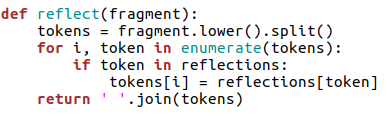
\includegraphics[scale=0.6]{./Pictures/reflect.png}
\caption{Reflect} 
\end{figure}

The first function that appears to us is called reflect. We iterate through the list of tokens and, if the token exists in our dictionary, we replace it with the value from the dictionary.

\begin{figure}[h]
\centering
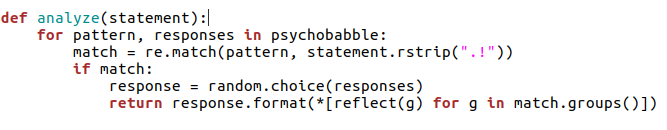
\includegraphics[scale=0.6]{./Pictures/analyze.png}
\caption{Analyze}
\label{fig:analyze}
\end{figure}

The second function that appears is called analyze. We look for if any word in the dictionary match with any word in the user's statement, from which we have stripped the final punctuation. If we find a match, we choose a response template randomly from the list of possible responses associated with the matching pattern. If not, we ask for more information.
\begin{figure}[h]
\centering
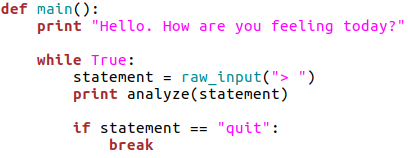
\includegraphics[scale=0.6]{./Pictures/main.png}
\caption{Main}
\label{fig:main}

\end{figure}
Finally, we have the main function that runs the program. First, we show the initial sentence on the screen, to begin the conversation with the user. From there and until the user does not want to stop, we continue having a conversation with him and analyzing his answers with the function presented in figure \ref{fig:analyze}.\\

Here is an example of a the output of the program:



\begin{figure}[h]
\centering
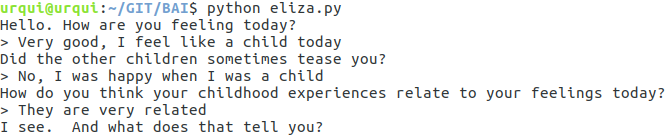
\includegraphics[scale=0.6]{./Pictures/example.png}
\caption{Example}
\end{figure}

We see that the program designed by Mr. Joseph Weizenbaum was nothing more than a very simple program with a program that responded according to previously created templates. With the creation of this program we could already see the first brushstrokes of artficial intelligence in a chatbots.
 

\subsection{ALICE}
	\label{sec:alice}
	
	If we are talking about chatbots, we can not forget ALICE. As \cite{shawar2002comparison} says, ALICE( Artificial Linguistic Internet Computer Entity) is a robot that you can make chatting with it. ALICE knowledge is stored in AIML files. AIML is an abbreviation of The Artificial Intelligent Mark up Language that is a derivative of Extensible Mark up Language(XML). The next sections describe necessary information about AIML elements, its categories, how they are used in ALICE and Pattern Matching Algorithm.

\section{Types of chatbots}
\label{sec:types}

	\subsection{Sentimental-chatbots}
	\label{sec:sentimental}
	
	Why would we want to add sentiment analysis to our chatbot? The reasons can be several, like adjusting better to the topic of the conversation, getting more natural answers from our chatbot or maybe just develop a chatbot to tell us something to make us feel better, someone to be with in bad times or someone to share happiness with.
	
	But before we start talking about sentimental chatbots, let's talk about sentiment analysis.
	
		\subsubsection{Sentiment analysis}
		\label{sec::sentiment_analysis}
		
		Opinion mining is usually called also sentiment analysis. According to Bing Liu from the University of Illinois: \\
		
		\begin{center}
			\textit{"Given a set of evaluative text documents that contain opinions (or sentiments) about an object, opinion mining aims to extract attributes and components of the object that have been commented on in each document d $\in$ D and to determine whether the comments are positive, negative or neutral"} \cite{bingliu_sentiment_definition}.
		\end{center}
		
		In other words, we have some documents containing subjective information and our goal is to evaluate this information in order to assign a sentiment or positiveness value to each comment or document.\\
		
		As B. Pang and L. Lee say, there are several problems in the sentiment analysis \cite{sentiment_analysis_bpang_llee}:
		
		\begin{itemize}
			\item First of all, we have to determine which documents or webpages have relevant information for sentiment analysis, that's opinions, reviews, etc.
			\item Then it comes the problem of which portions of the documents or the information we are analyzing are useful for the sentiment analysis.
			\item After this we have to determine whether the opinion or information expresses a positive or negative feeling, or directly with what feeling it corresponds. In some pages like 
					Amazon it can be easier since in the comments section, each comment is associated with a product evaluation that usually reflects the user's agreement and therefore the degree of positivity of the comment, but in other occasions in which we have no clue can be complicated.
			\item Finally we must internally represent in our chatbot or sentiment analysis program that feeling, since not in all the web pages or documents in which we are given a previous
				 	valuation the same measurement system is used (Amazon uses a 5 stars system, Yahoo answers uses a like-dislike system, etc) and we must normalize these values.
		\end{itemize}
	
		There are many tools that allow us or help us to analyze sentiment easily. Most of them are convolutional neural networks trained with huge datasets.
		
		We can use tools as a help for our algorithms in sentiment analysis such as "Tweet sentiment application" \footnote{https://www.csc2.ncsu.edu/faculty/healey/tweet\_viz/tweet\_app/} developed by Dr. Christopher Healey that allows you to search for tweets based on keywords and shows us information about tweets containing those keywords that can be very useful such as Sentiment, Topics, Heatmap, Tag Cloud, Timeline, Map, Affinity, Narrative and tweets. \\
		
		The most useful for us is the Sentiment information that show us a graphic representation of the sentiments shown in the tweets: \textit{"Sentiment. Each tweet is shown as a circle positioned by sentiment, an estimate of the emotion contained in the tweet's text. Unpleasant tweets are drawn as blue circles on the left, and pleasant tweets as green circles on the right. Sedate tweets are drawn as darker circles on the bottom, and active tweets as brighter circles on the top. Hover your mouse over a tweet or click on it to see its text"} \cite{tweet_sentiment_analysis}.
			
		\begin{figure}[h]
			\centering
			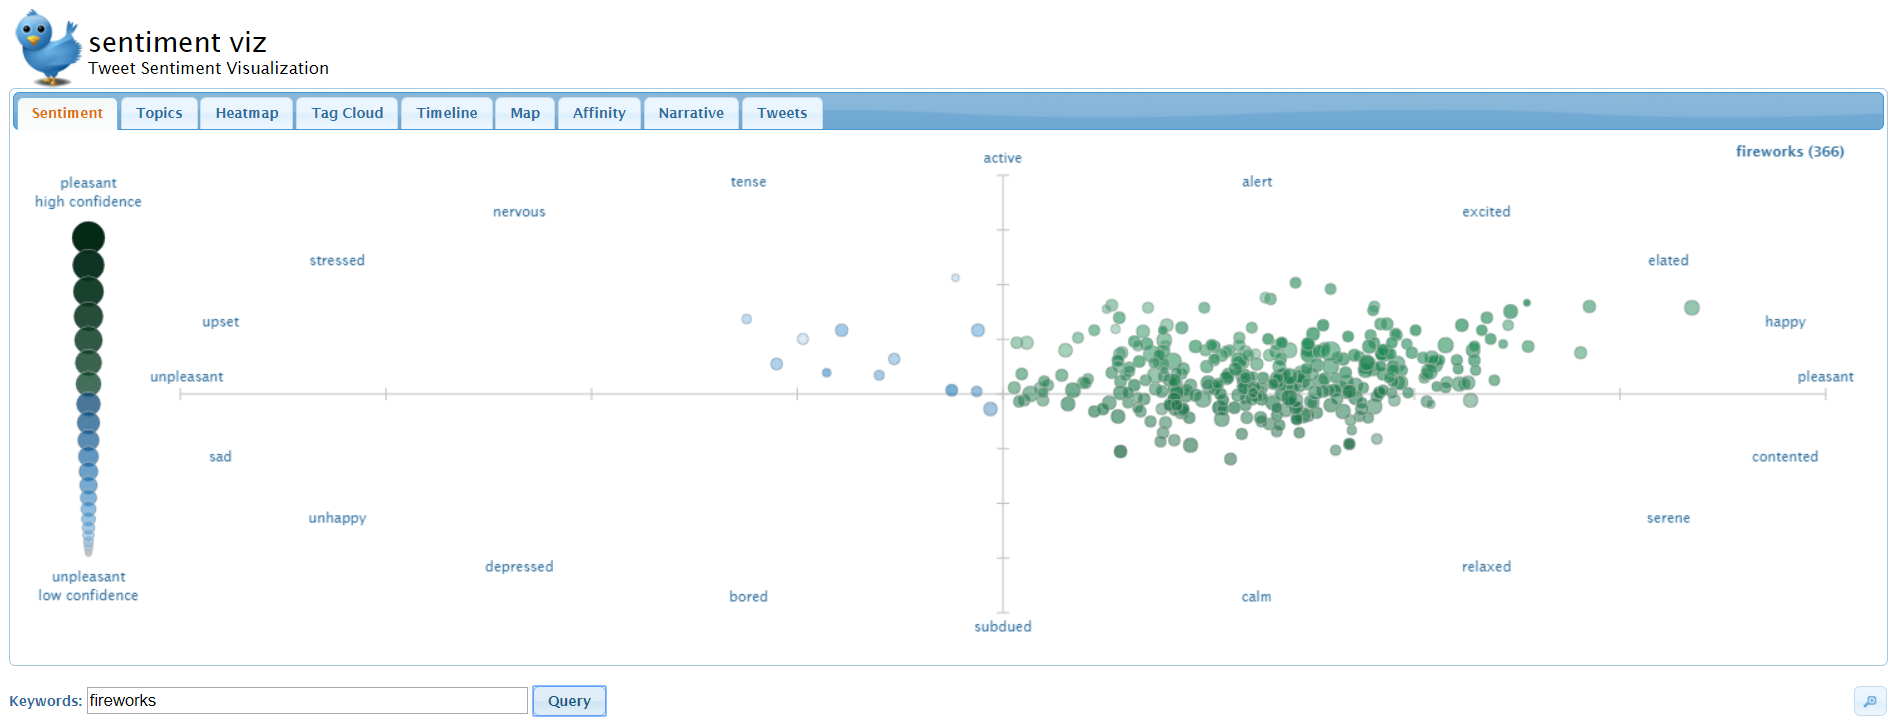
\includegraphics[scale=0.35]{./Pictures/fireworks_sentiment_visualization.png}
			\caption{As we can see, most of the tweets associated to the keyword "fireworks" are positive. This can be usefull when parsing some texts containing some words we don't know how to proccess.} 
		\end{figure}
	
		There are more general tools that we can use directly in our sentiment analysis like "pattern.en".
		
		\textit{"The pattern.en module contains a fast part-of-speech tagger for English (identifies nouns, adjectives, verbs, etc. in a sentence), sentiment analysis, tools for English verb conjugation and noun singularization \& pluralization, and a WordNet interface."} \cite{python_module}
		
		\begin{figure}[h]
			\centering
			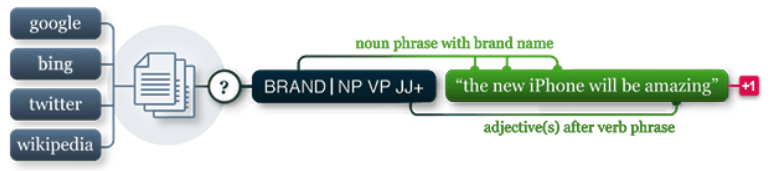
\includegraphics[scale=0.8]{./Pictures/python_module.png}
			\caption{Ilustration of the patter.en python module working.} 
		\end{figure}
	
		Let's take a deeper look into the sentiment section of this module. This module has two functions for sentyment analysis \cite{python_module_sentiment}:
		
		\begin{itemize}
			\item sentiment(sentence): It's the main function for sentiment analysis in this module . As we can read in the webpage \cite{python_module_sentiment}, it gives us two values:
			
			\begin{itemize}
				\item polarity: It takes values from -1.0 to 1.0. It tell us if the sentence is positive or negative. The algorithm is based on the adjectives of the sentence.
				\item subjectivity: It takes values from 0.0 to 1.0.
			\end{itemize}
			
			\item positive(s, threshold=0.1): It returns True if the given sentence's polarity is above the threshold. We can use this function to detect stronger ir lighter sentiments giving different values to the threshold. \textit{"Accuracy is about 75\% for movie reviews" }\cite{python_module_sentiment} so we can see that there are good tools free-to-use in our sentiment analysis. 
		\end{itemize}
		
		In another example, Cicero Nogueira dos Santos and Maira Gatti propose a deep convolutional neural network for sentiment analysis of short texts \cite{glorot2011domain}.\\
		
		In this case the neural network takes a sentence as an input and returns a score for each sentiment label in a set. 
		
		In order to do that, every word is converted into a vector, which is composed of two sub-vectors:
		
		\begin{itemize}
			\item Word-level: It captures syntactic and semantic information,
			\item Wharacter-level: It captures morphological and shape information.

		\end{itemize}
		
	 
		
		
		
	
		
	

	\subsection{Information-chatbots}
	\label{sec:information}

	\subsection{Game-chatbots}
	\label{sec:game}

	\subsection{Assistant-chatbots}
	\label{sec:assistant}
	

\section{Comparison of chatbots}
\label{sec:comparison}


\section{Chatbots in time}
\label{sec:time}

\subsection{Obsolets}
\label{sec:obsolet}

\subsection{Nowdays}
\label{sec:nowdays}

\subsection{Future}
\label{sec:future}

\section{Conclusion}
\label{sec:conclusion}

We have learned that

%%%%%%%%%%%%%%%%%%%%%%%%%%%%%%%%%%%%%%
% hier werden - zum Ende des Textes - die bibliographischen Referenzen
% eingebunden
%
% Insbesondere stehen die eigentlichen Informationen in der Datei
% ``bib.bib''
%
\nocite{*}


\newpage
\bibliographystyle{alpha}
\addcontentsline{toc}{section}{Bibliography}% Add to the TOC
\bibliography{bib}

\end{document}


